\begin{frame}[fragile]\frametitle{Procesamiento de una señal}
  \begin{center}
    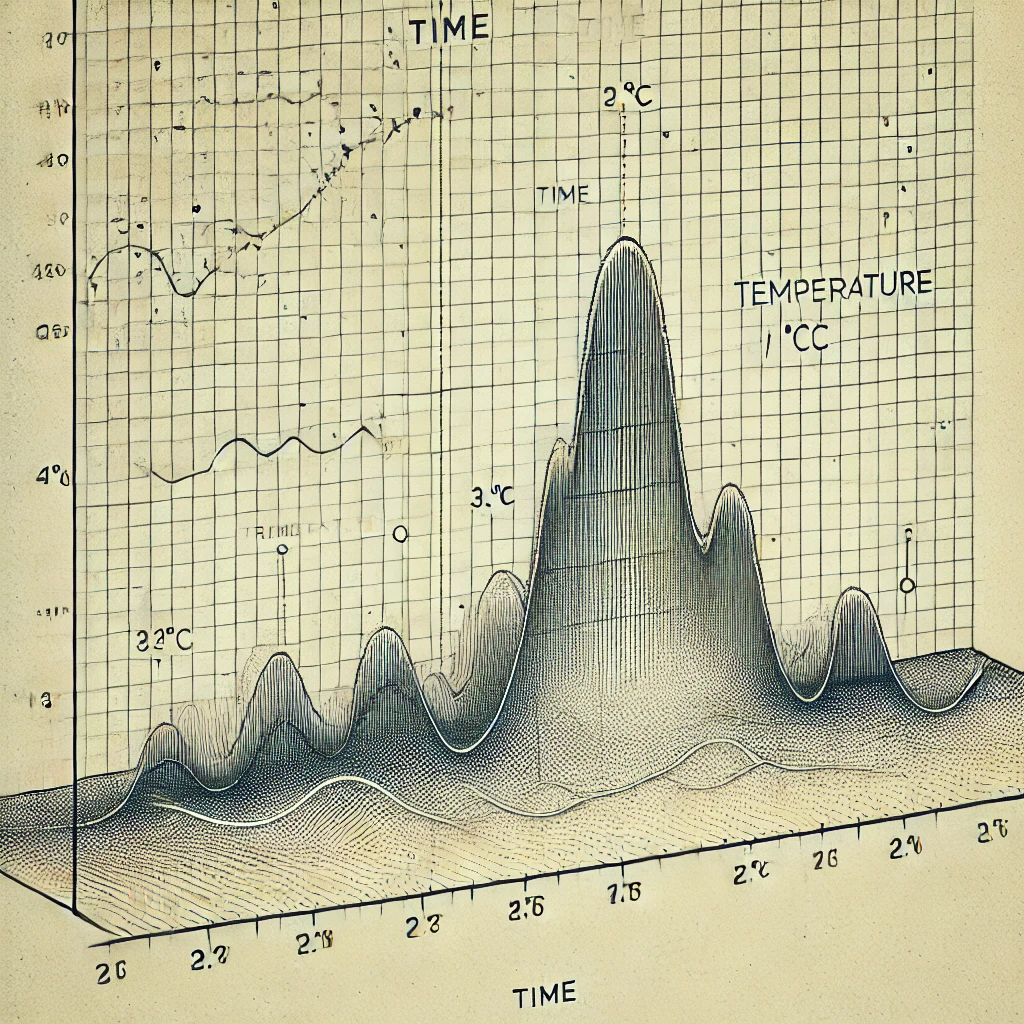
\includegraphics[width=3.5cm]{Figures/TemperatureSignal.png}
    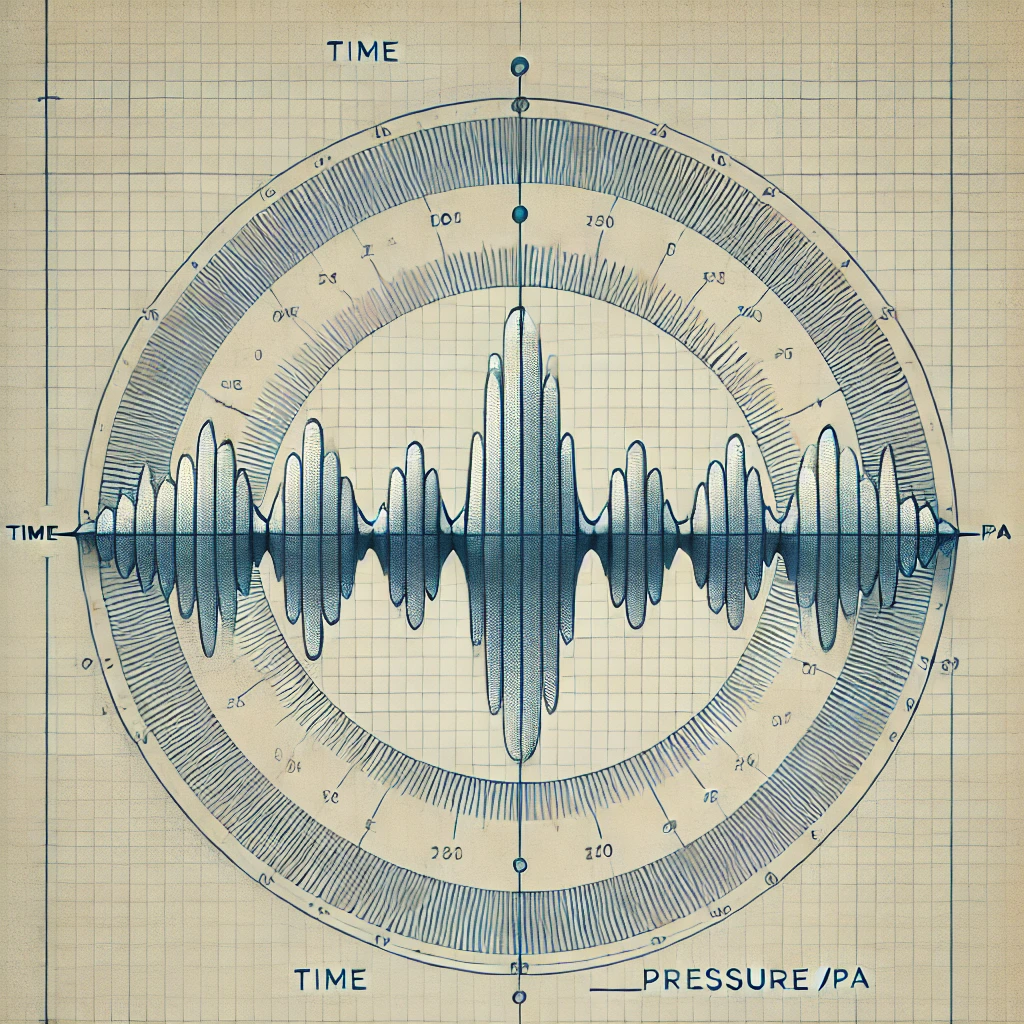
\includegraphics[width=3.5cm]{Figures/SoundPressure.png}
    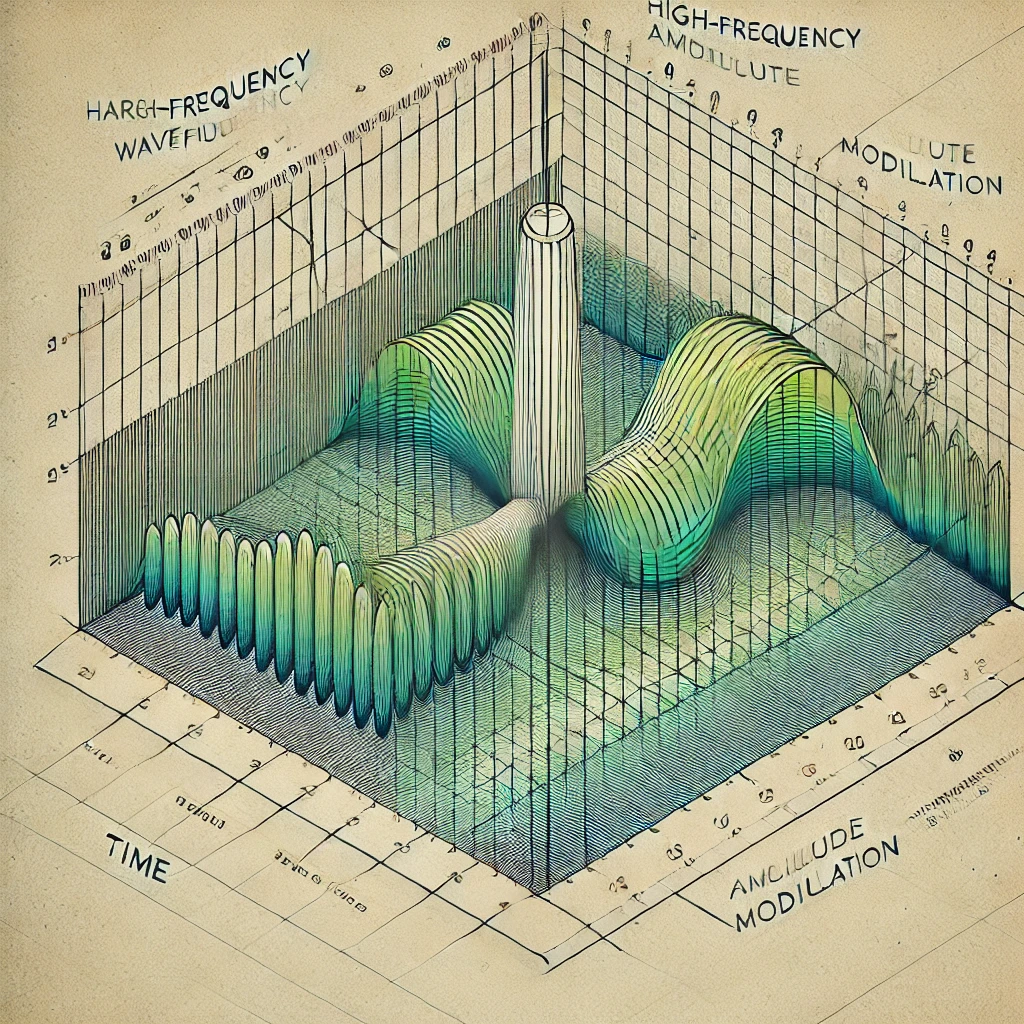
\includegraphics[width=3.5cm]{Figures/Radio.png}
  \end{center}
  \begin{itemize}
    \item Las señales provenientes del mundo real habitualmente son analógicas:
    \begin{itemize}
      \item Temperatura.
      \item Sonido (ondas de presión sonora).
      \item Señales de radio (ondas electromagnéticas).
    \end{itemize}
  \end{itemize}
\end{frame}

\begin{frame}\frametitle{Procesadores de señales}
  \begin{figure}
    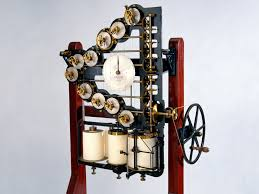
\includegraphics[height=2.5cm]{Figures/mareas.jpg}
    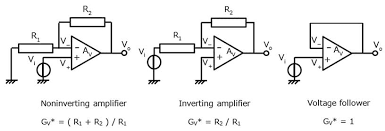
\includegraphics[height=2.5cm]{Figures/opamp.png}
  \end{figure}
  \begin{itemize}
    \item Los primeros procesadores de señales eran analógicos \href{https://www.youtube.com/watch?v=IgF3OX8nT0w}{(ver vídeo)}:
    \begin{itemize}
      \item Predictor de Mareas (Lord Kelvin, 1873).
      \item Moduladores/demodulares para comunicaciones.
      \item Filtros analógicos.
      \item Amplificadores operacionales (1939).
      \begin{itemize}
        \item Operaciones: suma, resta, integración, derivación...
        \item Filtros
      \end{itemize}
    \end{itemize}
    \item Algunas ventajas:
    \begin{itemize}
      \item Velocidad de procesamiento.
    \end{itemize}
    \item Algunas desventajas:
    \begin{itemize}
      \item Sensible al ruido.
      \item Poco flexible.
    \end{itemize}
  \end{itemize}
\end{frame}

\begin{frame}\frametitle{Procesadores de señales}
  \begin{center}
    \begin{tikzpicture}
      % Nodes
      \node (input) [] {};
      \node (adc) [block, right=0.8cm of input] {\tiny A/D};
      \node (dsp) [block, right=0.8cm of adc] {\tiny Procesador digital};
      \node (dac) [block, right=0.8cm of dsp] {\tiny D/A};
      \node (output) [right=0.8cm of dac] {};
      % Arrows
      \draw [arrow] (input) -- (adc) node[midway, above] {\tiny $x(t)$};
      \draw [arrow] (adc) -- (dsp) node[midway, above] {\tiny $x_d[n]$};
      \draw [arrow] (dsp) -- (dac) node[midway, above] {\tiny $y_d[n]$};
      \draw [arrow] (dac) -- (output) node[midway, above] {\tiny $y_a(t)$};
    \end{tikzpicture}
  \end{center}
  \begin{itemize}
    \item El auge de la electrónica digital plantea un enfoque alternativo.
    \begin{itemize}
      \item Convertir la señal continua en discreta mediante el muestreo.
      \item Procesar digitalmente.
      \item Reconstruir una señal continua a partir de las muestras procesadas. 

    \end{itemize}
    \item Algunas ventajas:
    \begin{itemize}
      \item Mayor flexibilidad.
      \item Menos sensible al ruido.
    \end{itemize}
    \item Algunas desventajas:
    \begin{itemize}
      \item Menor velocidad/latencia.
      \item Rango dinámico limitado.
    \end{itemize}
  \end{itemize}
\end{frame}

\begin{frame}\frametitle{Procesadores de señales}
  \begin{center}
    \begin{tikzpicture}
      % Nodes
      \node (input) [] {};
      \node (adc) [block, right=0.8cm of input] {\tiny A/D};
      \node (dsp) [block, right=0.8cm of adc] {\tiny Procesador digital};
      \node (dac) [block, right=0.8cm of dsp] {\tiny D/A};
      \node (output) [right=0.8cm of dac] {};
      % Arrows
      \draw [arrow] (input) -- (adc) node[midway, above] {\tiny $x(t)$};
      \draw [arrow] (adc) -- (dsp) node[midway, above] {\tiny $x_d[n]$};
      \draw [arrow] (dsp) -- (dac) node[midway, above] {\tiny $y_d[n]$};
      \draw [arrow] (dac) -- (output) node[midway, above] {\tiny $y_a(t)$};
    \end{tikzpicture}
  \end{center}
  \begin{itemize}
    \item Procesamiento digital de señales
    \begin{itemize}
      \item Algunos hitos históricos:
      \begin{itemize}
        % \item 1805 - Gauss (\emph{¡Cómo no!}): algoritmo precursor de la FFT\footnote{Aunque no lo publico en vida, según investigaciones recientes se le atribuye a Gauss (\emph{¡Cómo no!}) un algoritmo para el cálculo de coef. de SF finitas considerado el precursor de lo que hoy conocemos como FFT.}
        \item 1807, 1811 - Publicación resultados sobre series de Fourier\footnote{Según investigaciones recientes se le atribuye a Gauss (\emph{¡Cómo no!}), aunque no lo publico en vida, un algoritmo para el cálculo de coef. de SF finitas considerado el precursor de lo que hoy conocemos como FFT.}
        % \item 1821 - Primer ordenador digital: máquina diferencial de \emph{Babbage}
      %   % \item 1946 - ENIAC \emph{Electrical Numerical Integrator and Calculator}
        % \item 1947 - Invención del transistor (\emph{Bardeen}, \emph{Brattain} y \emph{Shockley})
        \item 1965 - Cooley \& Tukey: algoritmo FFT (Fast Fourier Transform)
        \item 1978 - INTEL lanza el 2920: procesador de señales analógicas
        \item 1982 - Texas Instruments lanza el TMS32010\\
        \hspace{1cm}{\scriptsize Primer procesador digital de señales (DSP) propiamente dicho}\\
        \hspace{1.5cm}{\scriptsize \color{blue}$\bullet$ \color{black} Arquitectura Harvard: datos e instrucciones separados}\\
        \hspace{1.5cm}{\scriptsize \color{blue}$\bullet$ \color{black} Operaciones MAC (Multiply-Accumulate)}\\
      \end{itemize}
    \end{itemize}
  \end{itemize}
\end{frame}


\begin{frame}[fragile]\frametitle{Procesador Digital de Señales (DSP)}
  \begin{tikzpicture}
    % Nodes
    \node (input) [] {};
    \node (antialiasing) [block, right=1cm of input] {\begin{minipage}{1.25cm}\centering\setlength{\baselineskip}{1.5em}\tiny Filtro\\ anti-aliasing\end{minipage}};
    \node (adc) [block, right=0.8cm of antialiasing] {\tiny A/D};
    \node (dsp) [block, right=0.8cm of adc] {\tiny Procesador digital};
    \node (dac) [block, right=0.8cm of dsp] {\tiny D/A};
    \node (smoothing) [block, right=0.8cm of dac] {\begin{minipage}{1.25cm}\centering\setlength{\baselineskip}{1.5em}\tiny Filtro de\\suavizado\end{minipage}};
    \node (output) [right=0.8cm of smoothing] {};
    % Arrows
    \draw [arrow] (input) -- (antialiasing) node[midway, above] {\tiny $x(t)$};
    \draw [arrow] (antialiasing) -- (adc) node[midway, above] {\tiny $x_a(t)$};
    \draw [arrow] (adc) -- (dsp) node[midway, above] {\tiny $x_d[n]$};
    \draw [arrow] (dsp) -- (dac) node[midway, above] {\tiny $y_d[n]$};
    \draw [arrow] (dac) -- (smoothing) node[midway, above] {\tiny $y_a(t)$};
    \draw [arrow] (smoothing) -- (output) node[midway, above] {\tiny $y(t)$};
  \end{tikzpicture}
  \begin{itemize}
    \item \alert{Esquema general:}
    \begin{itemize}\scriptsize
      \item El filtro antialiasing garantiza una señal de ancho de banda limitado.
      \item El ADC convierte la señal analógica en una señal digital.
      \item El procesador digital realiza la manipulación de la señal.
      \item El DAC convierte la señal digital en una señal analógica.
      \item El filtro de suavizado elimina las altas frecuencia debidas a la reconstrucción.
    \end{itemize}
  \end{itemize}
\end{frame}


\begin{frame}\frametitle{Muestreo, cuantificación y codificación}
  \footnotesize
  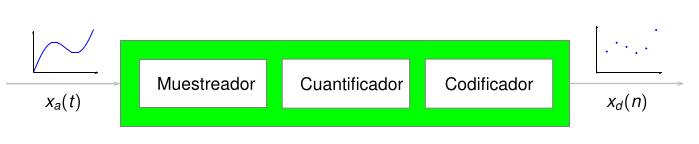
\includegraphics[width=\textwidth]{Figures/MCC.png}
  \begin{itemize}
    \item \textbf{Muestreo}: Es la conversión de una señal analógica $x_a(t)$ en una señal de tiempo discreto x(n). Consiste en tomar ``muestras'' de la señal continua $x_a(t)$ en ciertos instantes de tiempo: $x(n)=x_a(t=t_n)$.
    \item \textbf{Cuantificación}\visible<5->{$^{1}$}: Es la conversión de una señal de tiempo discreto $x(n)$ que toma valores continuos en una señal de tiempo discreto que toma también valores discretos, es decir en una señal digital $x_d(n)$.
    \item \textbf{Codificación}: Cada valor digital $x_d(n)$ se representa mediante una secuencia binaria \{011011101010101\}.
  \end{itemize}
  \rule{5cm}{0.4pt}\scriptsize\\
  $^1$ El muestreo y la cuantificación pueden realizarse en orden inverso. En la práctica siempre se realizan asi. 
\end{frame}


